\documentclass[reprint,english,notitlepage]{revtex4-2}

\usepackage[utf8]{inputenc}
\usepackage[english]{babel}

\usepackage{physics,amssymb}
\usepackage{graphicx}
\usepackage{xcolor}
\usepackage{hyperref}
\usepackage{tikz}
\usepackage{listings}
\usepackage{subfigure}
\usepackage{placeins}
\graphicspath{ {/Users/rebeccanguyen/Documents/GitHub/H22} }

\hypersetup{
    colorlinks,
    linkcolor={red!50!black},
    citecolor={blue!50!black},
    urlcolor={blue!80!black}}


\lstset{
	inputpath=,
	backgroundcolor=\color{white!88!black},
	basicstyle={\ttfamily\scriptsize},
	commentstyle=\color{magenta},
	language=Python,
	morekeywords={True,False},
	tabsize=4,
	stringstyle=\color{green!55!black},
	frame=single,
	keywordstyle=\color{blue},
	showstringspaces=false,
	columns=fullflexible,
	keepspaces=true}

\begin{document}
\title{Temperfect mug}   % self-explanatory
\author{Rebecca Nguyen}               % self-explanatory
\date{\today}                             % self-explanatory
\noaffiliation
\maketitle                                % creates the title, author, date & abstract


% the fundamental components of scientific reports:
\section{Introduction}
In this experiment we want to study the temperature of a liquid in two thermos mugs; Bodum and Temperfect.
Bodum mug is a regular thermos cup. The Temperfect mug extracts excess heat from your beverage and stores it in its walls. This allows the newly-brewed beverage to
be enjøyed right away. In the walls of this mug is a layer of insulation which changes from solid to liquid as it absorbs heat. Thereafter, the heat is used to keep
the beverage at a perfect temperature and the material returns to a solid state.
We will be looking at temperature development over time for both mug. Both in order to see if the mug works as advertised and discuss if Temperfect can be modelled
as an Einstein solid.

\section{Theory}
The multiplicity in an Einstein solid is given by
\begin{equation}
  \Omega(N, q) = \frac{(q+N -1)!}{q! (N -1)!} \approx \frac{(q+N)!}{q!N!}
\end{equation}
where q is number of energy units $\epsilon$ and N is number of oscillators. The expression has been further simplified using Stirling's approximation. We have considered the case q $\gg$ N (when there are
more energy units than oscillators, the so-called 'high-temperature' limit) in order to simplify it.
This gives us the expression for entropy
\begin{equation}
  S \equiv k \ln\Omega
\end{equation}
where k is Boltzmann's constant.
Internal energy of an Einstein solid is given by

\begin{equation}
  U = \frac{N}{2}\epsilon + q\epsilon
\end{equation}

Which results in
\begin{equation}
  \frac{dU}{dq} = \epsilon \rightarrow dU = \epsilon dq
\end{equation}
with variations in.\\

One of the most important identities in thermal dynamics, derived from the first law of thermodynamics, is as follows
\begin{equation}
dU = Tds - Pdv \\
\end{equation}
We assume constant pressure and volume which allows us to rewrite the equation as
\begin{equation}
  dU = Tds \rightarrow T = \frac{dU}{dS} = \frac{\epsilon dq}{dS}
\end{equation}
Numerically we find this as
\begin{equation}
  T_i = \epsilon\frac{q_i - q_{i -1}}{S_i - S_{i -1}}
\end{equation}
\\
Lastly we have heat capacity
\begin{equation}
C_v = \frac{dU}{dT} = \frac{\epsilon dq}{dT}
\end{equation}
Numerically we find this as
\begin{equation}
  C_{v, i} = \epsilon\frac{q_i - q_{i -1}}{T_i - T_{i -1}}
\end{equation}

\section{Method}
The Temperfect mug and Bodum thermos cup were both filled with 3dl of almost boiling water. The lids were not put on to allow temperature logging while the water in the mugs cooled. The temperature in the air outside of the mug was $T_a = 22^{\circ}$.
\begin{figure}[!htb]
  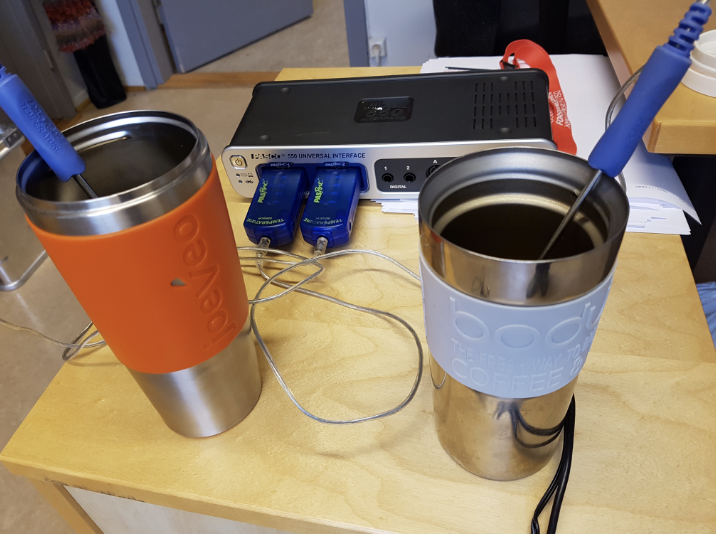
\includegraphics[scale=0.5]{setup.png}
  \caption{Experimental setup for comparing the Temperfect and Bodum mug}\label{fig:setup}
\end{figure}
\FloatBarrier

\section{Results}
In figure (\ref{fig:temperature}) we have plotted temperature of both thermal mugs against time. Based on this figure we can conclude with Temperfect being mug 2 and Bodum being mug 1. The reasoning for this is mug 2's ability to bring the beverage temperature from almost boiling to a comfortable temperature rather fast. Based on the orange graph, the temperature stay in the so-called 'Ahhh zone' for a longer period
\begin{figure}
  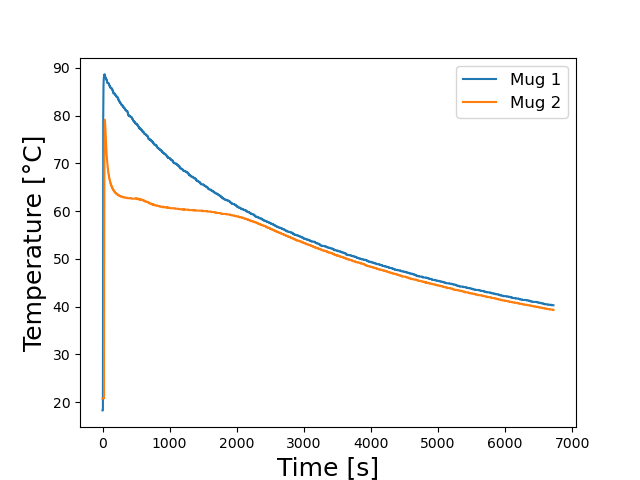
\includegraphics[scale=0.5]{temp.png}
  \caption{Temperature against time of both mugs}\label{fig:temperature}
\end{figure}
\FloatBarrier


\begin{figure}
  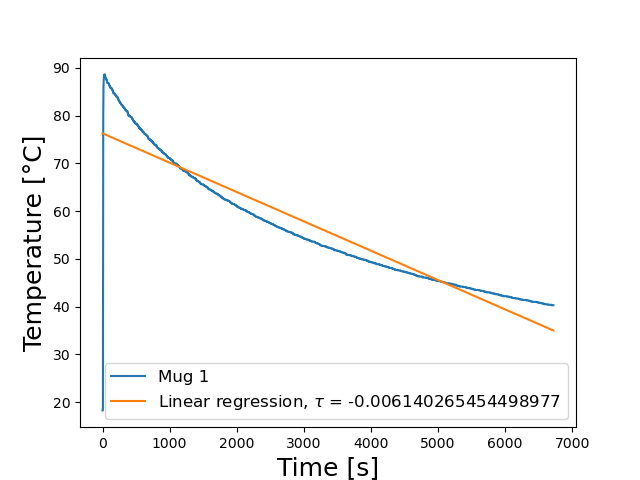
\includegraphics[scale=0.5]{tau_t.png}
  \caption{}\label{fig:tau_t}
\end{figure}
\FloatBarrier

\begin{figure}
  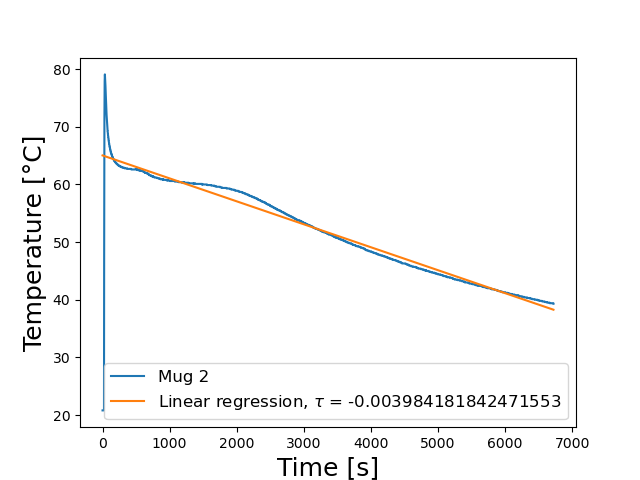
\includegraphics[scale=0.5]{tau_b.png}
  \caption{}\label{fig: tau_b}
\end{figure}
\FloatBarrier

\section{Discussion and conclusion}




%% When it comes to the bibliography I personally generate it using BibLaTeX. (see the link above if you're interested)
%% You're obviously allowed to create the references section however you like.
%% I'll keep it simple here.
\section*{References}  % the asterisk (*) after \section makes the section numbering go away
\begin{itemize}
\item[-]Reference 1
\item[-]Reference 2
\end{itemize}

\newpage
%% if you want to include an appendix, this is how you do it
\appendix
\section{Name of appendix}
This will be the body of the appendix.


\end{document}
